\subsection{A8}\label{A8}

Kappa architecture is similar to Lambda but it has one big difference: it excludes batch processing. Arguably, it can be called another version of real time processing. If there is a batch of files send to it, they are handled as a stream of data \parencite{feick2018fundamentals}.

Since Kappa is similar to real time processing, lets reuse roller coaster example. In batch processing, we would wait for 20 people to fill the ride before operator would start the ride. In Kappa, people would still queue for the ride but as soon as the ride is available all of the people who are there would be ready to ride. In other words, our roller coaster would operate real time with the goal of less stopping regardless how many people are on the ride.

As mentioned with the real time processing, this is something that could be used with flamingo data. For example, instead of waiting for conversation between players to finish, they can directly be processed.

\begin{figure}[H]
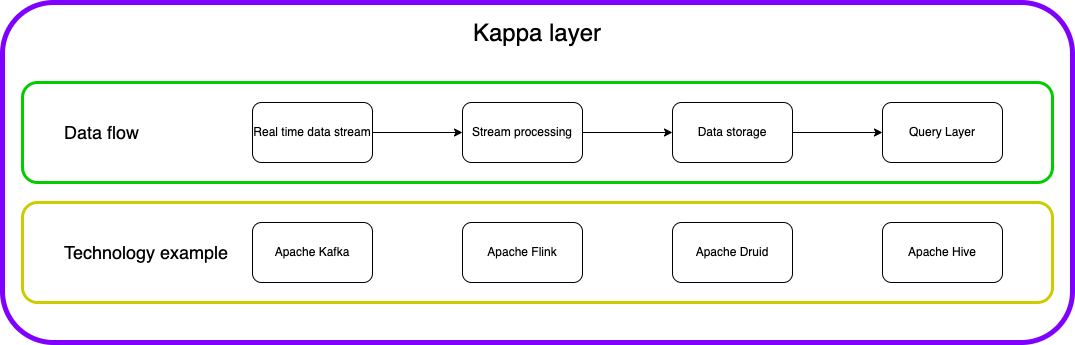
\includegraphics[scale=0.35]{img/ProcessingParadigms/BigData-Kappa.png}
\centering
\caption{Kappa}
\label{fig:Kappa}
\end{figure}